\documentclass[11pt]{article}
\oddsidemargin -.2in
\evensidemargin -.2in
\topmargin -.2in
\textwidth 6.9in
\textheight 8.7in
%%%%%%%%%%%%%%%%%%%%%%%%%

\usepackage[parfill]{parskip}    % Activate to begin paragraphs with an empty line rather than an indent
\usepackage{latexsym, amssymb, bbm}
\usepackage{amsmath}
\usepackage{amsfonts}
\usepackage{amsthm}
\usepackage{verbatim}
\usepackage{fancyhdr}
\usepackage{enumerate}
\usepackage{mathtools}
\usepackage{graphicx}
\usepackage{dsfont}
\usepackage{float}

%%%%%%%%%%%%%%%%%%%%%%%%%

\newtheorem{thm}{Theorem}[section]
\newtheorem{lem}[thm]{Lemma}
\newtheorem{prop}[thm]{Proposition}
\newtheorem{cor}[thm]{Corollary}
\newtheorem{cla}[thm]{Claim}
\newtheorem{con}[thm]{Conjecture}

\theoremstyle{definition}
\newtheorem*{defn}{Definition}
\newtheorem{example}[thm]{Example}
\newtheorem{axiom}{Axiom}
\newtheorem*{note}{Note}
\newtheorem*{question}{Question}

\theoremstyle{remark}
\newtheorem{case}{Case}

%%%%%%%%%%%%%%%%%%%%%%%%%
%%%%%%%%%%%%%%%%%%%%%%%%%%
%%%%%%%% EDIT HERE %$%%%%%%%%%
%%%%%%%%%%%%%%%%%%%%%%%%%%%%
%%%%%%%%%%%%%%%%%%%%%%%%%%%%%

\newcommand{\name}{Casper Neo}
\newcommand{\classname}{Introduction to Econometrics: Honors}
\newcommand{\classnumber}{ECON 209}
\newcommand{\due}{15 March 2017}
\newcommand{\num}{}
\newcommand{\type}{Immigration and Inequality}

%%%%%%%%%%%%%%%%%%%%%%%%%%%%%
%%%%%%%%%%%%%%%%%%%%%%%%%%%%
%%%%%%%%%%%%%%%%%%%%%%%%%%%
%%%%%%%%%%%%%%%%%%%%%%%%%%
%%%%%%%%%%%%%%%%%%%%%%%%%
\pagestyle{fancy}
\lhead{\name}
\chead{\classnumber\space\space-\space\type\space\num}
\rhead{\due}

%-------------------------------------------------------


%-------------------------------------------------------

\newcommand{\lecture}[1]{\centerline{\fbox{\textbf{#1}}}}
\newcommand{\que}[2] {\vspace{.25in} \fbox{#1} #2 \vspace{.10in}}
\renewcommand{\part}[1] {\vspace{.10in} {\bf (#1)}}


%%%%%%%%%%%%%%%%%%%%%%%%%%

% SHORTCUTS FOR BLACKBOARD BOLD
\def\C{\mathbb{C}}
\def\N{\mathbb{N}}
\def\Q{\mathbb{Q}}
\def\R{\mathbb{R}}
\def\Z{\mathbb{Z}}
\def\1{\mathbb{1}}
\def\P{\mathbb{P}}
\def\0{\emptyset}

% SHORTCUTS FOR MATH BOLD FONT
\def\ba{\mathbf{a}}
\def\bb{\mathbf{b}}
\def\be{\mathbf{e}}
\def\bf{\mathbf{f}}
\def\bh{\mathbf{h}}
\def\bu{\mathbf{u}}
\def\bv{\mathbf{v}}
\def\bx{\mathbf{x}}
\def\by{\mathbf{y}}
\def\bz{\mathbf{z}}
\def\bzero{\mathbf{0}}
\def\bone{\mathbf{1}}

% SHORTCUTS FOR GREEK LETTERS
\def\a{\alpha}
\def\b{\beta}
\def\g{\gamma}
\def\G{\Gamma}
\def\d{\delta}
\def\D{\Delta}
\def\e{\varepsilon}
\def\k{\kappa}
\def\l{\lambda}
\def\m{\mu}
\def\r{\rho}
\def\s{\sigma}
\def\t{\tau}
\def\th{\theta}
\def\x{\xi}
\def\vp{\varphi}
\def\n{\nabla}
\def\w{\omega}
\def\z{\zeta}
\def\vp{\varphi}
\def\p{\phi}
\def\Ph{\Phi}
\def\L{\Lambda}
\def\Si{\Sigma}
\def\Th{\Theta}
\def\O{\Omega}

\def\el{\ell}

% SHORTCUTS FOR MATH SCRIPT
\def\sR{\mathscr{R}}
\def\sA{\mathscr{A}}
\def\sC{\mathscr{C}}
\def\sM{\mathscr{M}}
\def\sF{\mathscr{F}}
\def\sB{\mathscr{B}}
\def\sL{\mathscr{L}}

% SHORTCUTS FOR MATH CAPITALS
\def\A{\mathcal{A}}
\def\cC{\mathcal{C}}
\def\cE{\mathcal{E}}
\def\cF{\mathcal{F}}
\def\cH{\mathcal{H}}
\def\cL{\mathcal{L}}
\def\cM{\mathcal{M}}
\def\cP{\mathcal{P}}
\def\cU{\mathcal{U}}


\def\i{^{-1}}
\newcommand{\fin}{f^{-1}}
\def\lp{\mathop{\rm lp}}
\def\slp{\mathop{\rm slp}}
\def\ext{\mathop{\rm ext}}
\def\sep{\mathop{\rm sep}}
\def\rel{\mathop{\rm rel}}
\def\lub{\mathop{\rm lub}}
\def\glb{\mathop{\rm glb}}

\def\ds{\displaystyle}

\newcommand{\lpvar}[1]{\,\textrm{lp}_{#1}\,}
\newcommand{\ol}[1]{\overline{#1}}
\newcommand{\fl}[1]{\left\lfloor #1 \right\rfloor}
\newcommand{\cl}[2]{\left\lceil \frac{#1}{#2} \right\rceil}
\newcommand{\md}[1]{(\text{mod } #1)}
\newcommand{\cs}[1]{\begin{case} #1 \end{case}}
\newcommand{\abs}[1]{\left\lvert #1 \right\rvert}
\newcommand{\norm}[1]{\lVert#1\rVert}
\newcommand{\set}[1]{\{ #1 \}}
\DeclarePairedDelimiter{\ceil}{\lceil}{\rceil}
\DeclarePairedDelimiter{\floor}{\lfloor}{\rfloor}


\newcommand{\upint}[2]{
  \overline{\int_{#1}^{#2}}
}
\newcommand{\loint}[2]{
  \underline{\int_{#1}^{#2}}
}

\DeclareMathOperator{\spn}{span}
\DeclareMathOperator{\diam}{diam}
\DeclareMathOperator*{\E}{\mathbb{E}}
\DeclareMathOperator*{\pr}{\mathbb{P}}

\newenvironment{piecewise}{\left\lbrace
\begin{matrix}}
{
\end{matrix}
\right.
}

\def\defeq{\stackrel{\tt{\tiny def}}=}

\def\la{\langle}
\def\ra{\rangle}

\def\ben{\begin{enumerate}}
\def\een{\end{enumerate}}

\def\ptl{\partial}
\newcommand{\pd}[2]{\frac{\ptl#1}{\ptl #2}}

\def\tt{\text}
\def\tb{\textbf}
\def\pipe{|}
\def\Sin{\tt{sin}}
\def\^{\wedge}
\def\del{\nabla}
\def\iid{\stackrel{iid}\sim}

% SHORTCUTS FOR LIMITS
\def\ltx{\lim_{t\to x}}
\def\lxp{\lim_{x\to p}}
\def\lxa{\lim_{x\to a}}
\def\lni{\lim_{n\to\infty}}
\def\lsni{\limsup_{n\to\infty}}
\def\lxi{\lim_{x\to\infty}}
\def\lxz{\lim_{x\to0}}
\def\lhz{\lim_{h\to0}}
\def\ltz{\lim_{t\to0}}

% SHORTCUTS FOR SUMMATIONS
\def\sion{\sum_{i=1}^n}
\def\sjon{\sum_{j=1}^n}
\def\sjom{\sum_{j=1}^m}
\def\snoi{\sum_{n=1}^\infty}
\def\sioi{\sum_{i=1}^\infty}
\def\snzi{\sum_{n=0}^\infty}
\def\snzN{\sum_{n=0}^N}
\def\skoi{\sum_{k=1}^\infty}
\def\siok{\sum_{i=1}^k}
\def\skon{\sum_{k=1}^n}
\def\skzn{\sum_{k=0}^n}
\def\pion{\prod_{i=1}^n}

% SHORTCUTS FOR INTEGRALS
\def\ipp{\int_{-\pi}^\pi}
\def\iii{\int_{-\infty}^{\infty}}
\def\izp{\int_0^\pi}
\def\iztp{\int_0^{2\pi}}
\def\izr{\int_0^r}
\def\izo{\int_0^1}
\def\ioi{\int_1^\infty}
\def\iab{\int_a^b}
\def\izi{\int_0^\infty}
\def\riea{\sR(\a)}
\newcommand{\eval}[2]{\Big\vert_{#1}^{#2}}

% SHORTCUTS FOR ENVIRONMENTS
\newcommand{\al}[1]{\begin{align*}#1\end{align*}}
\newcommand{\aleq}[1]{\begin{equation}\begin{aligned}[b]#1\end{aligned}\end{equation}}
\newcommand{\bigb}[1]{\bigg(#1\bigg)}
\newcommand{\prf}[1]{\begin{proof}#1\end{proof}\vspace{3mm}}
\newcommand{\bmtx}[1]{\begin{bmatrix}#1\end{bmatrix}}
\newcommand{\enum}[2]{\begin{enumerate}[#1]#2\end{enumerate}}
\newcommand{\pwise}[1]{\begin{piecewise}#1\end{piecewise}}
\newcommand{\inm}[1]{\norm{#1}_2}
\newcommand{\enviro}[2]{\begin{#1}#2\end{#1}}
\newcommand{\tabler}[2]{\begin{center}\begin{tabular}{#1}#2\end{tabular}\end{center}}

\newcommand{\seq}[2]{\{#1_#2\}}

%%%%%%%%%%%%%%%%%%%%%%%%%%%%%%%%%%%%%%%%%%%%%%%%

\begin{document}
%--------------------------------------------------------------
\title{
	\vspace{-10mm}
    \classnumber\\
	\classname\\
    \type \space \num\\
}
\author{
	\name
}
\date{
	\due\\
}

\maketitle
%--------------------------------------------------------------

\section{Introduction}

This article is my final project in ECON 209: Honors Econometrics.
It is a partial replication and extension of David Card's
\textit{Immigration and Inequality}. Like in Card's paper, I estimate the
elasticity of substitution between education and income groups using a constant
elasticity of substitution (CES) model and linear regression.
Special attention on selective inference and multiple testing
corrections will be applied to bound the false discovery rate and false coverage
rates.


\renewcommand{\baselinestretch}{0.9}\normalsize
\tableofcontents
\listoffigures
\listoftables
\renewcommand{\baselinestretch}{1.0}\normalsize

\pagebreak
\section{Original Paper}

\textit{Immigration and Inequality} by David Card was published in 2009 in the
American Economic Review. It explores the relationship between immigration
status, education, and wages. Card uses the 1980-2000 Census data combined with
the 2005-2006 American Community Survey data. In contrast I use the 2007-2015
American Community Survey. Card explores his hypothesis with time series and
panel data as well. I select from his paper the following hypothesis to
test and replicate.

\begin{enumerate}
    \item Workers with below high school education are perfect substitutes
    for those with a high school education.

    \item High school-equivalent and college-equivalent workers are imperfect
    substitutes with an elasticity of substitution between 1.5-2.5;

    \item Within education groups, immigrants and natives are imperfect
    substitutes.
\end{enumerate}

As a main criticism which I will attempt to address is the fact that Card explores
multiple hypothesis and does not address the fact that potentially many more hypothesis
were considered (implicitly or otherwise) but not included in his paper. For example
he may have checked the elasticity of substitution between immigrants and natives,
grouped by race, geography or decade of entry.

\section{Data Overview}

Data from `https://www.census.gov/programs-surveys/acs/data/pums.html'.

I download the 1-year ACS surveys from 2007-2015 however only few columns
are used. I identified the following variables as relevant from the
\textit{PUMS Data Dictionary 2011-2015}. I map these variables from the
values in the raw data into units usable by my models.
Between the 8 years there are 27'725'196 people surveyed.
Though after I filter for working age (18-60) and those in the labor force
there are 11'994'312 people.
The procedure and models are developed a random 5\% sample then run
on the remaining 95\%.


\begin{table}[H]
    \caption{Data Used }
    \vspace{5mm}
    \label{}
    \centering
    \begin{tabular}{| l | l |}
        \hline
        Variable Key    & Description \\
        \hline \hline

        WAGP            & Wages or salary income past 12 months \\
        CIT             & Citizenship status \\
        NATIVITY        & Native or Foreign Born \\
        AGEP            & Age \\
        SCHL            & Years of Schooling \\
        ESR             & Employment Status Recode \\
        DECADE          & Decade of entry into the United States \\
        ST              & State \\
        \hline
    \end{tabular}
\end{table}


\section{Multiple Testing Concerns and Selective Inference}

When the same dataset is used to generate hypothesis as the dataset used to
test the hypothesis, researchers run into a multiple testing problem where, while
generating their model, they  mentally filter out models that seem not to fit the
data and in the end use models that fit well. It is then little surprise that the
models chosen have a strong fit to the data. Since both the question and the
answer to the question are functions of (and so are dependent on) the same data,
knowing the question reveals information about the answer; i.e. the hypothesis
and the resulting p-values or confidence intervals are not independent. The
simplest resolution to this is to use different data to generate the hypothesis
and to test the hypothesis. Hence, while I am using more recent data than David
Card, whose hypothesis I test, I write my procedure using a random partition of
my data and run tests on the rest.

I apply the Benjamini Hochberg False Discovery Rate (BH-FDR) control
algorithm to bound the false discovery rate when studying the elasticity of
substitution between groups. This has been shown  to work when the
test statistics are independent or exhibit positive regression dependancy. Since
I am comparing the elasticity of substitution between groups. This assumption
is probably valid. If education changes the elasticity of substitution for
natives, intuitively it should do so for immigrants as well due to similar
effects on marginal productivity.

Let $n$ be the number of p-values, and $\a$ the false discovery rate
you want to guarantee. The algorithm is to first find $k^*$ such that
$$k^* = \max\{k :\text{at least }k\text{ p-values } < \a\frac kn\}$$
Then reject the $k^*$ smallest p-values. By adjusting the threshold
with $k$, the procedure accounts for both many weak signals and few strong
signals. The procedure also comes with a simple process for constructing confidence
intervals such that false coverage rate is controlled. Simply construct
$(1-\a\frac{k^*}n)$ confidence intervals.

The advantage of this procedure over the well known Bonferroni correction is
power at the cost of flexibility. The Bonferroni procedure does not assume anything
about the distribution or correlation of p-values however it is too conservative
and only the stongest of signals will reject a null hypothesis. The BH-DFR
procedure takes advantage of positive dependance and also rejects null hypothesis
when there are many weak signals. However a drawback is that while
expected proportion of discoveries that are false is bounded, the variance of
the proportion grows with positive correlation.

\section{Estimating Elasticity of Substitution Between Groups}

Assuming a 1 sector framework with a Constant Elasticity of Substitution (CES)
model

\begin{equation}
    y = [\a_J L_{J^\r} + \a_K L_{K^\r}]^{\frac 1\r}
\end{equation}

Where $J$ and $K$ are separate groups (for example high school educational
equivalents and college equivalents), $\r = 1-\frac1\s$ and $\s$ is the
between group elasticity of substitution.
$L$ is the labor input, estimated by $1-$ the unemployment rate within the group.
Observe as $\r\to 1$, $\s \to \infty$, a percent change in group $J$'s labor
input corresponds to infinite change in group $K$'s labor input. That is, they
are perfect substitutes.
When $\r\to-\infty$, $\s \to 0$ which means every percent change in group $J$'s
labor input should correspond to a percent change in group $K$'s labor input.
That is, they are perfect complements.
When $\r = 0$, $\s = 1$ we reach the threshold at which if $\r \downarrow$
then $\s\downarrow$ and we have complements, and if $\r\uparrow$ then $\s \uparrow$
and we have substitutes. As a null hypothesis I assume $\s=1$ so we may test
if the groups are substitutes or complements.

 $\r = 1$, $\s = \infty$ and we have perfect substitutes. As
$\r\to\-\infty$ we have $\s \to 1$ which means every percent change in group $J$'s
labor input should correspond to a percent change in group $K$'s labor input.
That is, they are perfect complements. As a null hypothesis for arbitrary groups
I will assume they are perfect substitutes and $\s = \infty$.
This production function may be estimated by the the linear model

\begin{equation}
    \log \frac{w_j}{w_k} = \log\frac{\a_j}{\a_k} - \frac 1\s \log\frac{L_j}{L_k}
\end{equation}

We observe labor inputs, and wages then use a linear model to estimate
$\s = \frac 1{\b_1}$. Our data has sufficient detail to know if the observed
is a non-citizen, naturalized citizen, or born citizen (the former two are
considered immigrants). We can also distinguish years of education, which state
and even public use micro-data area code (By the census definition).
The latter designate areas of 100'000 or more population.
Each data point in the CES model is over one micro-data area in one year.
If one of the groups is empty (which is possible given a large number of public
micro-data areas, years, and categories) a divide by zero error will be reached.
I throw out such data points and any $x,y$ pairs with infinite values.
Given the granularity of my data there are many potential hypothesis attempting
to find the elasticity of
substitution split along the following lines;

\begin{itemize}
    \item Immigrant vs native
    \item Non-citizen vs citizen
    \item Non-citizen vs naturalized citizen
    \item Non-citizen vs born citizen
    \item Naturalized citizens vs born citizens
    \item less than high school educated vs only high school educated
    \item less than high school educated vs college educated
    \item less than high school educated vs at least high school educated
    \item high school educated vs college educated
    \item less than college educated vs college educated.
\end{itemize}

25 more hypothesis splitting across education while fixing citizenship
and 25 more hypothesis splitting across citizenship while fixing education.
I choose these 60 hypothesis since they seem the most natural. Their corresponding
data are generated algorithmically and are listed in Section 8. 

With a set of 3 education levels there are 7 ways to include education levels
in groups. Analogously for citizenship levels. Hence there are 49 potential groups.
That means when comparing the elasticity of substitution between groups there are
$${(2^3-1) * (2^3-1) \choose 2} = {49\choose 2} = 1176$$
ways to split the data
of varying degrees of reasonability. The combinatoric explosion gets exponentially
worse if I also chose to include race, decade of entry, geography, or any other
potential categories.


\section{Conclusion and Results}

After running, for every hypothesis;$H^1,...,H^{60}$; a two sided $T-$test testing
the null $H_0^i:\b^{H^i}_1 = 1$ we get 60 p values. We run the $BH-FDR$ procedure
and find 33 nulls were rejected while 27 were not. A surprising number of nulls
where rejected however this is more to do with the dependance between the
overlapping hypothesis.

Of the 33 rejections, we find 26 of them are considered gross substitutes while
7 of them are considered compliments. Interestingly, since I generated the
hypothesis automatically we a kind of structure in the hypothesis space.
Odd numbered hypothesis are comparing citizenship level groups
(immigrant vs born citizen or non-citizen vs citizen) while holding level of
education constant. For hypothesis $H^{37},H^{39},H^{41},H^{43}$ which correspond
to Card's conclusion; that within education groups, immigrants and natives
are imperfect substitutes with a large but finite elasticity of substitution;
we fail to reject the null hypothesis that that $\s=1$.




\begin{figure}[H]
    \centering
    \caption{Slope Parameter}
    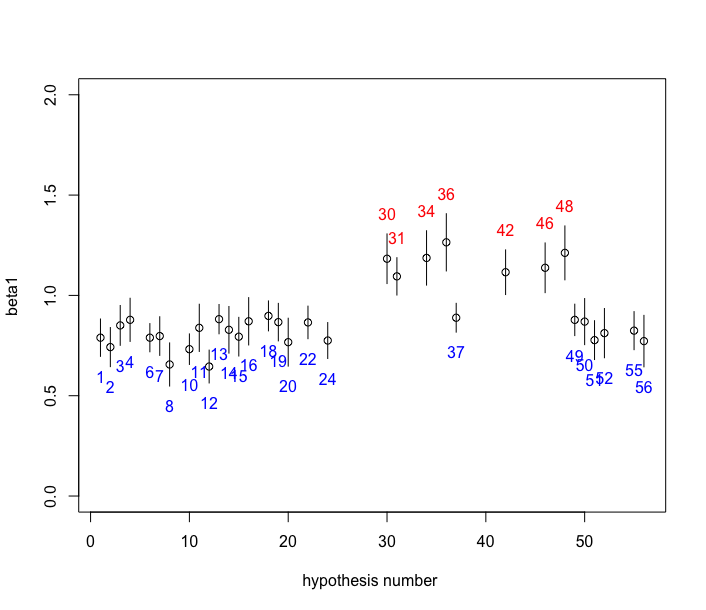
\includegraphics[width=.7\textwidth]{slopeFinal.png}

    \label{slo}
\end{figure}

\begin{figure}[H]
    \centering
    \caption{Elasticity of Substitution}
    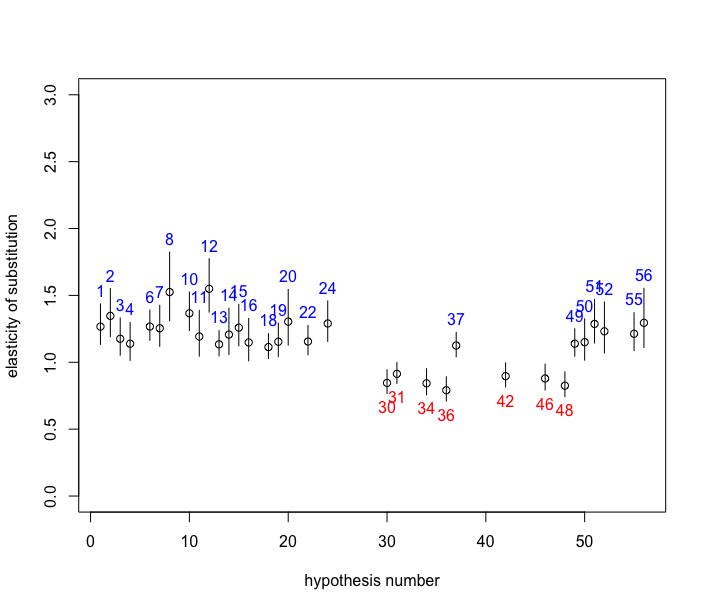
\includegraphics[width=.7\textwidth]{elasticityFinal.png}

    \label{est}
\end{figure}



\section{Appendix: My code}

Github link: https://github.com/CasperN/Immigration-and-Inequality.git

To download and clean the data, run in a unix terminal \textit{bash getdata.sh}.
Note \textit{cleanData.py} should be in the same directory when this happens.
This will automatically download and clean the data as I use it, and randomly
split the data into a set for hypothesis generation and another for testing.

\textit{generateHypothesis.py} will read either the training or testing data
then process the data into simple $x$s and $y$s to be compared in a simple
linear model. These data are saved in a \textit{hypothesis/} directory.
\textit{analysis.R} reads the hypothesis and performs the multiple testing
corrections.


\begin{thebibliography}
\small
    \bibitem{C} Card, David. 2009. "Immigration and Inequality." American Economic Review, 99(2): 1-21. http://www.aeaweb.org/articles?id=10.1257/aer.99.2.1

    \bibitem{B} Benjamini, Yoav; Yekutieli, Daniel. The control of the false discovery rate in multiple testing under dependency. Ann. Statist. 29 (2001), no. 4, 1165--1188. doi:10.1214/aos/1013699998. http://projecteuclid.org/euclid.aos/1013699998.
\end{thebibliography}



\section{Appendix: 60 Plausible sounding null hypothesis}

\setlength{\parskip}{0em}

\tiny{
H1: For below high school workers, the elasticity of substitution between non-citzens and naturalized citizens is $\infty$

H2: For non-citizen workers, the elasticity of substitution between below high school and high school equivalent education is $\infty$

H3: For high school equivalent workers, the elasticity of substitution between non-citzens and naturalized citizens is $\infty$

H4: For naturalized citizen workers, the elasticity of substitution between below high school and high school equivalent education is $\infty$

H5: For college equivalent workers, the elasticity of substitution between non-citzens and naturalized citizens is $\infty$

H6: For born citizen workers, the elasticity of substitution between below high school and high school equivalent education is $\infty$

H7: For below college workers, the elasticity of substitution between non-citzens and naturalized citizens is $\infty$

H8: For immigrant workers, the elasticity of substitution between below high school and high school equivalent education is $\infty$

H9: For high school or more workers, the elasticity of substitution between non-citzens and naturalized citizens is $\infty$

H10: For all citizen workers, the elasticity of substitution between below high school and high school equivalent education is $\infty$

H11: For all workers, the elasticity of substitution between non-citzens and naturalized citizens is $\infty$

H12: For all workers, the elasticity of substitution between below high school and high school equivalent education is $\infty$

H13: For below high school workers, the elasticity of substitution between non-citizens and born citizens is $\infty$

H14: For non-citizen workers, the elasticity of substitution between below high school and college equivalent is $\infty$

H15: For high school equivalent workers, the elasticity of substitution between non-citizens and born citizens is $\infty$

H16: For naturalized citizen workers, the elasticity of substitution between below high school and college equivalent is $\infty$

H17: For college equivalent workers, the elasticity of substitution between non-citizens and born citizens is $\infty$

H18: For born citizen workers, the elasticity of substitution between below high school and college equivalent is $\infty$

H19: For below college workers, the elasticity of substitution between non-citizens and born citizens is $\infty$

H20: For immigrant workers, the elasticity of substitution between below high school and college equivalent is $\infty$

H21: For high school or more workers, the elasticity of substitution between non-citizens and born citizens is $\infty$

H22: For all citizen workers, the elasticity of substitution between below high school and college equivalent is $\infty$

H23: For all workers, the elasticity of substitution between non-citizens and born citizens is $\infty$

H24: For all workers, the elasticity of substitution between below high school and college equivalent is $\infty$

H25: For below high school workers, the elasticity of substitution between naturalized and born citizens is $\infty$

H26: For non-citizen workers, the elasticity of substitution between high school equivalent and college equivalent education is $\infty$

H27: For high school equivalent workers, the elasticity of substitution between naturalized and born citizens is $\infty$

H28: For naturalized citizen workers, the elasticity of substitution between high school equivalent and college equivalent education is $\infty$

H29: For college equivalent workers, the elasticity of substitution between naturalized and born citizens is $\infty$

H30: For born citizen workers, the elasticity of substitution between high school equivalent and college equivalent education is $\infty$

H31: For below college workers, the elasticity of substitution between naturalized and born citizens is $\infty$

H32: For immigrant workers, the elasticity of substitution between high school equivalent and college equivalent education is $\infty$

H33: For high school or more workers, the elasticity of substitution between naturalized and born citizens is $\infty$

H34: For all citizen workers, the elasticity of substitution between high school equivalent and college equivalent education is $\infty$

H35: For all workers, the elasticity of substitution between naturalized and born citizens is $\infty$

H36: For all workers, the elasticity of substitution between high school equivalent and college equivalent education is $\infty$

H37: For below high school workers, the elasticity of substitution between immigrants and born citizens is $\infty$

H38: For non-citizen workers, the elasticity of substitution between below college and college equivalent education is $\infty$

H39: For high school equivalent workers, the elasticity of substitution between immigrants and born citizens is $\infty$

H40: For naturalized citizen workers, the elasticity of substitution between below college and college equivalent education is $\infty$

H41: For college equivalent workers, the elasticity of substitution between immigrants and born citizens is $\infty$

H42: For born citizen workers, the elasticity of substitution between below college and college equivalent education is $\infty$

H43: For below college workers, the elasticity of substitution between immigrants and born citizens is $\infty$

H44: For immigrant workers, the elasticity of substitution between below college and college equivalent education is $\infty$

H45: For high school or more workers, the elasticity of substitution between immigrants and born citizens is $\infty$

H46: For all citizen workers, the elasticity of substitution between below college and college equivalent education is $\infty$

H47: For all workers, the elasticity of substitution between immigrants and born citizens is $\infty$

H48: For all workers, the elasticity of substitution between below college and college equivalent education is $\infty$

H49: For below high school workers, the elasticity of substitution between non-citizens and citizens is $\infty$

H50: For non-citizen workers, the elasticity of substitution between below and above high school education is $\infty$

H51: For high school equivalent workers, the elasticity of substitution between non-citizens and citizens is $\infty$

H52: For naturalized citizen workers, the elasticity of substitution between below and above high school education is $\infty$

H53: For college equivalent workers, the elasticity of substitution between non-citizens and citizens is $\infty$

H54: For born citizen workers, the elasticity of substitution between below and above high school education is $\infty$

H55: For below college workers, the elasticity of substitution between non-citizens and citizens is $\infty$

H56: For immigrant workers, the elasticity of substitution between below and above high school education is $\infty$

H57: For high school or more workers, the elasticity of substitution between non-citizens and citizens is $\infty$

H58: For all citizen workers, the elasticity of substitution between below and above high school education is $\infty$

H59: For all workers, the elasticity of substitution between non-citizens and citizens is $\infty$

H60: For all workers, the elasticity of substitution between below and at or above high school education is $\infty$
}


%------------------------------------------------------------------------------------------------------------
\end{document}
